\documentclass[UTF8]{beamer}
\usefonttheme[onlymath]{serif}
\setbeamertemplate{navigation symbols}{}
\usetheme{CambridgeUS}
%\setbeamerfont{text}{family*={ptm}, shape=\upshape, series=\mdseries}

\title{An Introduction to Polkadot}
\author{Wang Kaixuan}
\institute[SJTU]{Shanghai Jiao Tong University}

\usepackage{subfigure}

\newcommand{\Setup}{\textsf{\textit{Setup}}}
\newcommand{\Eval}{\textsf{\textit{Eval}}}
\newcommand{\Verify}{\textsf{\textit{Verify}}}
\newcommand{\SNKGen}{\textsf{\textit{SNKGen}}}
\newcommand{\SNKProve}{\textsf{\textit{SNKProve}}}
\newcommand{\SNKVerify}{\textsf{\textit{SNKVerify}}}
\newcommand{\IVCGen}{\textsf{\textit{IVCGen}}}
\newcommand{\IVCProve}{\textsf{\textit{IVCProve}}}
\newcommand{\IVCVerify}{\textsf{\textit{IVCVerify}}}
\newcommand{\Prime}{\textsf{\textit{Prime}}}

\newcommand{\pp}{\mathbf{pp}}
\newcommand{\poly}{\textsf{\textit{poly}}}
\newcommand{\negl}{\textsf{\textit{negl}}}

\newcommand{\cA}{\mathcal{A}}
\newcommand{\cB}{\mathcal{B}}
\newcommand{\cC}{\mathcal{C}}
\newcommand{\cD}{\mathcal{D}}
\newcommand{\cE}{\mathcal{E}}
\newcommand{\cF}{\mathcal{F}}
\newcommand{\cG}{\mathcal{G}}
\newcommand{\cH}{\mathcal{H}}
\newcommand{\cI}{\mathcal{I}}
\newcommand{\cJ}{\mathcal{J}}
\newcommand{\cK}{\mathcal{K}}
\newcommand{\cL}{\mathcal{L}}
\newcommand{\cM}{\mathcal{M}}
\newcommand{\cN}{\mathcal{N}}
\newcommand{\cO}{\mathcal{O}}
\newcommand{\cP}{\mathcal{P}}
\newcommand{\cQ}{\mathcal{Q}}
\newcommand{\cR}{\mathcal{R}}
\newcommand{\cS}{\mathcal{S}}
\newcommand{\cT}{\mathcal{T}}
\newcommand{\cU}{\mathcal{U}}
\newcommand{\cV}{\mathcal{V}}
\newcommand{\cW}{\mathcal{W}}
\newcommand{\cX}{\mathcal{X}}
\newcommand{\cY}{\mathcal{Y}}
\newcommand{\cZ}{\mathcal{Z}}

\newcommand{\bG}{\mathbb{G}}
\newcommand{\bN}{\mathbb{N}}
\newcommand{\bZ}{\mathbb{Z}}

\newcommand{\leftdollar}{\xleftarrow{\text{\tiny$\mathsf{\$}$}}}

\begin{document}
	\usebeamerfont{text}
	\begin{frame}
		\titlepage
	\end{frame}

	\begin{frame}{Introduction}
		\begin{block}{Polkadot}
			Polkadot utilizes a central chain called the relay chain which communicates with multiple heterogeneous and independent sharded chains called parachains.\\
			I
		\end{block}
	\end{frame}

	\begin{frame}{Substrate}
		\begin{block}{What is Substrate?}
			Substrate is an open source, modular, and extensible framework for building  blockchains.
		\end{block}
		\begin{block}{}
			Substrate provides the core components of a blockchain: 
			\begin{enumerate}
				\item Database Layer
				\item Networking Layer
				\item Transaction Queue
				\item Consensus Engine
				\item Framework for Runtime Development
			\end{enumerate}
		Each of Which can be customized and extended
		\end{block}
	\end{frame}

	\begin{frame}{The Substrate Runtime}
		\begin{columns}
			\column{0.5\textwidth}
			\begin{block}{Runtime}
				\begin{enumerate}
					\item The runtime is the \textbf{block execution logic} of the blockchain, a.k.a the State Transition Function.
					\item It is composed of FRAME Pallets
				\end{enumerate}
			\end{block}
			\bigskip
			\bigskip
			\bigskip
			\bigskip
			\column{0.5\textwidth}
			\begin{figure}
				\centering
				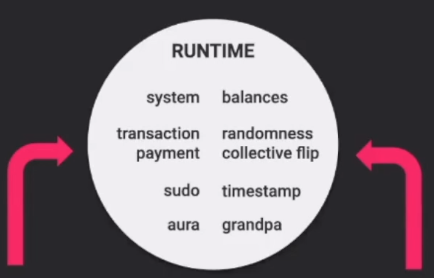
\includegraphics[width=6cm]{figure/Runtime}
				\centering
				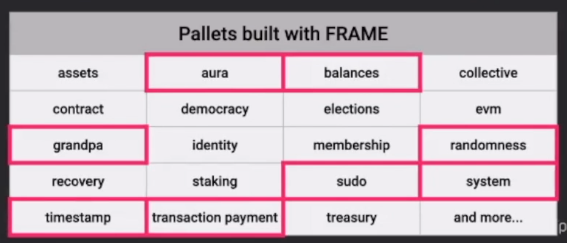
\includegraphics[width=6cm]{figure/Runtime2}
				\caption{Runtime and Frame}
			\end{figure}
		\end{columns}
	\end{frame}

	\begin{frame}{Building Blocks of Substrate}
		\begin{figure}
			\centering
			\includegraphics[width=0.7\linewidth]{"figure/Building Blocks of substrate"}
			\caption{}
			\label{fig:building-blocks-of-substrate}
		\end{figure}
	\end{frame}

	\begin{frame}{Why WebAssembly}
		\begin{block}{}
		Wasm is a platform independent executable format
		\begin{itemize}
			\item Wasm is Sandboxed
			\item Wasm is Fast
			\item Wasm is Compact
			\item Wasm is Well Supported
		\end{itemize}
	\end{block}
	\end{frame}
\end{document} 